\subsection{\textit{Backend for a Ticketing System}}

Tesis ini membahas desain sistem tiket. Tesis ini berfokus pada desain modul, fungsionalitas, serta relasi yang diperlukan untuk menjalankan sistem ini. Penelitian ini berbeda dengan penelitian sebelumnya yang fokus membahas desain dari sisi arsitektur \parencite{backendForTicketing}. Tesis ini tidak membahas arsitektur secara detil dan hanya membagi fungsionalitas menjadi beberapa modul. Oleh karena itu, arsitektur yang digunakan pada penelitian ini adalah arsitektur \textit{modular monolith}.

Terdapat empat entitas yang digambarkan pada sistem ini, yaitu:

\begin{enumerate}
    \item Pengguna yang bertugas untuk mencari dan membeli tiket, melakukan pembayaran, dan mengubah profil pengguna.
    \item Organisasi yang bertugas untuk mengatur acara, kategori tiket, dan lain-lain.
    \item Validator yang bertugas untuk memberi izin dan mencegah terjadinya pelanggaran yang berkaitan dengan validitas dan integritas tiket.
    \item Admin yang bertugas atas registrasi organisasi dan mengatur sertifikat penjual tiket.
\end{enumerate}

\pagebreak

Gambar \ref{fig:event-rm} dan Gambar \ref{fig:ticket-storage} menggambarkan diagram relasi entitas untuk \textit{events} dan entitas yang berkaitan pada proses pembuatan dan penyimpanan tiket.

\begin{figure}[htbp]
    \centering
    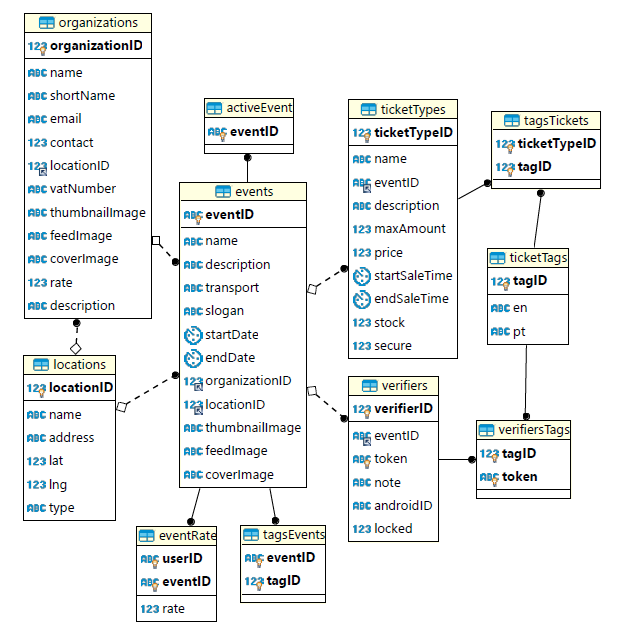
\includegraphics[width=0.6\textwidth]{resources/chapter-2/event-rm.png}
    \caption{ERD \textit{events} \parencite{backendForTicketing}}
    \label{fig:event-rm}
\end{figure}

\begin{figure}[htbp]
    \centering
    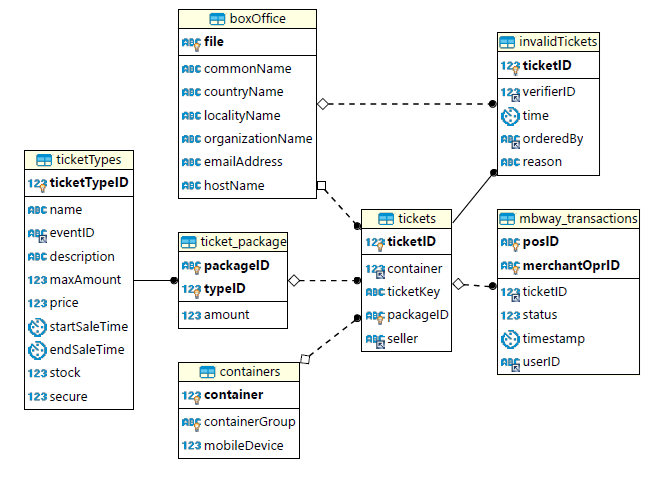
\includegraphics[width=0.6\textwidth]{resources/chapter-2/er-ticket-storage.png}
    \caption{ERD dengan entitas untuk pembuatan dan penyimpanan tiket \parencite{backendForTicketing}}
    \label{fig:ticket-storage}
\end{figure}

Tesis ini hanya membahas sistem dari aspek desain fitur dan entitas. Arsitektur sistem tidak dibahas secara detil. Selain itu, aspek skalabilitas dan toleransi kegagalan tidak dibahas pada tesis ini.